\chapter{Background} \label{chapt:Background}

In this chapter we provide background and related work for this thesis. Section \ref{background:setting} introduces the setting of this work in machine learning and data streams, including notation and definitions. Section \ref{background:related_work} discusses the related work on concept drift. Section \ref{background:conclusion} summarises the related work.

%-------------------------------------------------------------------
% SETTING
%-------------------------------------------------------------------

\section{Setting} \label{background:setting}

In this section we outline the setting of this thesis. Specifically, we provide the definitions and notation which will be used to describe machine learning and data streams.

% In Section \ref{setting:ml} we give notation and definitions relating to machine learning.  In Section \ref{setting:data_streams} we give notation and definitions relating to data streams.  

% \subsection{Machine Learning} \label{setting:ml}

% \newcommand{\y}[1]{y^{(#1)}}
% \newcommand{\yhat}[1]{\hat{y}^{(#1)}}
% \newcommand{\q}[1]{q^{(#1)}}
% \newcommand{\qhat}[1]{\hat{q}^{(#1)}}
\newcommand{\id}[1]{\mathds{1}[#1]} % identity function
\newcommand{\x}[1]{x^{(#1)}}
\newcommand{\X}[1]{X^{(#1)}}
% \newcommand{\qyhat}{\q{\hat{y}}}

A {\bf label} is a random variable to be predicted by the machine learning model, denoted $y\in dom(y)$. In general, a label may be (non-exhaustively) binary, numeric, or categorical. However, in this thesis we will only be concerned with binary and categorical labels.\footnote{An astute reader will note that we equivocate between $y$ being a random variable and $y$ being a specific value {\it of} that variable, and similarly with $x,q,z$, etc. This is to simplify notation.}  

A {\bf binary label} may only take the values $0$ and $1$. We will denote binary labels with $y$. Because this is also the symbol for a generic label, we will explicitly note when a label is binary. A {\bf multiclass label} may take on any of $n$ values, $dom(y)=\{c_1,c_2,\dots,c_n\}$. %We denote a multiclass label as a one-hot vector ${\bf y}=(y^{(1)},y^{(2)},\dots,y^{(n)})$, where $y^{(i)}=\id{y=c_i}$, and $\id{}$ is the identity function. For example, if $dom(y)=\{cats, dogs, pigeons\}$, and $y=pigeons$, then
% \begin{equation}
%     \bf{y} = \begin{pmatrix}y^{(0)}\\y^{(1)}\\y^{(2)}\end{pmatrix} = \begin{pmatrix}0\\0\\1\end{pmatrix}
% \end{equation}

An {\bf instance} is a vector concatenation of one or more variables called {\bf features}, and is denoted $x\in dom(x)$. Features may be (non-exhaustively) binary, numeric, categorical, or free text, and an instance may have any combination of feature types. The $n$-th feature of an instance is denoted $\x{n}$.

A {\bf concept} is a joint probability of instances and labels:
\begin{equation}
    \Pr(x,y).
\end{equation}
It is often convenient to express this in terms of a ``true" relationship between instances and labels, plus some amount of noise, as in:
\begin{equation}
    y = f(x) + \epsilon(x)
\end{equation}
where $f$ is the {\bf relationship}, and $\epsilon$ is {\bf noise} random variable which may or may not vary with $x$. 

The marginal probabilities of labels and instances are called the {\bf label distribution} and the {\bf instance distribution}, and denoted
\begin{equation}
    P(y) \text{ and } P(x).
\end{equation}
 
% The {\bf conditional label distribution} is the probability distribution over labels, conditional on the corresponding instance. For a binary label $y$, we denote conditional label distributions with
% \begin{equation}
%     q = \Pr(y=1|x).
% \end{equation}
% For a multiclass label we use
% \begin{equation}
%     \bf{q} = \begin{pmatrix}q^{(0)}\\q^{(1)}\\\vdots \\q^{(n)}\end{pmatrix} =\begin{pmatrix}\Pr(\y{0}=1|x)\\\Pr(\y{1}=1|x)\\ \vdots\\\Pr(\y{n}=1|x) \end{pmatrix}.
% \end{equation}
% Because the classes are mutually exclusive, we require
% \begin{equation}
%     \|{\bf q}\|_1=\sum_{i=0}^n \q{i} =1.
% \end{equation}
A {\bf learner} is an algorithm designed to infer from a set of instance label pairs a {\bf model} which approximates the relationship between instances and labels. The output of a model is called a {\bf prediction} and is denoted $\hat{y}$. 

There are two kinds of predictions we are concerned with. The first is a {\bf point prediction}, in which the model simply outputs the prediction $\hat{y}$.  
% \begin{equation}
%     \hat{y} = \hat{f}(x) \approx f(x)
% \end{equation}
% or in the multiclass case
% \begin{equation}
%     {\bf \hat{y}} = \hat{f}(x) =  \begin{pmatrix}\yhat{0}\\\yhat{1}\\ \vdots\\\yhat{n} \end{pmatrix} = \begin{pmatrix}\id{\hat{y}=c_0}\\\id{\hat{y}=c_1}\\ \vdots\\\id{\hat{y}=c_n} \end{pmatrix} = \hat{f}(x) \approx {\bf y}.
% \end{equation}
~The second is a {\bf probabilistic prediction}, in which the model outputs a probability distribution over possible labels. 

Due to noise, stochasticity, or the limited inferential capabilities of the learner, there is some probability that the model will make the wrong prediction. We thus denote
\begin{equation}
q = \Pr(y=\hat{y})
\end{equation}
as the {\bf reliability} of the model, or the probability that the model will make the correct prediction, for the given instance. 

For a model which makes probabilistic predictions, the {\bf confidence} is the probability assigned by the model to its predicted label, denoted
\begin{equation}
\hat{q} = \hat{\Pr}(y=\hat{y}).
\end{equation}
The {\bf residual} of a prediction is a metric of the disparity between predictions and labels. For our purposes, it is given by
\begin{equation}
    res = \id{y=\hat{y}} = \begin{cases} 1 & \text{if }y=\hat{y} \\ 0 & \text{if }y\ne\hat{y}.
    \end{cases}.
\end{equation}

% \begin{equation}
%     \hat{q} = \hat{f}(x) \approx \Pr(y=1|x).
% \end{equation}
% or in the multiclass case
% \begin{equation}
%     {\bf \hat{q}} = \hat{f}(x) =  \begin{pmatrix}\qhat{0}\\\qhat{1}\\ \vdots\\\qhat{n} \end{pmatrix} \approx {\bf q}.
% \end{equation}
% The {\bf risk} of a model is the probability of an incorrect prediction:
% \begin{equation}
%     R = P(y=\hat{y}) = \int P(\hat{y}\ne y|x)dP(x)
% \end{equation}
% where $\int f(x) dP(x)$ is the Lebesgue-Stieltjes integral. We use it for the convenience of indicating that $x$ may be discrete or continuous. If $y$ is a binary variable, then we have
% \begin{align}
%     P(\hat{y}\ne y|x) =& P(\hat{y}\ne f(x)=y|x) \\
%     &+ P(\hat{y}=f(x)\ne y|x).
% \end{align}
% The first term is {\bf reducible error}, and can be corrected with further learning. The second term is {\bf irreducible error} and cannot be corrected.

% \subsection{Data Streams} \label{setting:data_streams}

A {\bf time series} is a sequence of values which become successively available as time progresses. We denote these as
\begin{equation}
    Z = z_0,z_1,z_2,\dots
\end{equation}
A {\bf Bernoulli time series} consists of samples of a random variable where:
\begin{equation}
    z_i = \begin{cases}
    1 & \text{with probability $p$} \\
    0 & \text{with probability $1-p$}
    \end{cases}
\end{equation}
where $p$ is the {\bf rate} of the series. The rate of the residual series is called the {\bf error rate} of the model. 

The times at which each value in the time series becomes available are denoted by
\begin{equation}
    \tau_0,\tau_1,\tau_2,\dots
\end{equation}
If the differences in time between all instances are equal, or formally
\begin{equation}
    \tau_{i+1}-\tau_{i} = c
\end{equation}
for all $i\in\mathbb{N}$ and some constant $c$, then the time series is an {\bf evenly spaced time series}. Otherwise it is an {\bf unevenly spaced time series}. 

An example of an evenly spaced time series is hourly measurements of air quality \cite{ME}. An example of an unevenly spaced time series is our motivating example of GP referrals triage, in which new referral documents or clinician labels may become available at any time.

Some specific time series we are interested in are {\bf instance series} or {\bf feature series}, 
the {\bf label series},
the {\bf prediction series},
and the {\bf residual series}, which are denoted, respectively,
\begin{align}
    X &= x_0,x_1,x_2\dots \\
    Y &= y_0,y_1,y_2\dots \\
    \hat{Y} &= \hat{y}_0,\hat{y}_1,\hat{y}_2\dots \\
    RES &= res_0,res_1,res_2\dots
\end{align}
An instance time series and a label time series together are called a {\bf data stream}. A {\bf drift} is a change in the distribution of a series
\begin{equation}
    \Pr_t(z) \ne \Pr_{t+1}(z) \label{eq:drift}
\end{equation}
where $\Pr_t(z)$ is the distribution of $z$ at time $t$. The point at which a drift occurs is called a {\bf drift point} or {\bf drift location}. In Equation \ref{eq:drift}, the drift point is $t+1$.

% For a Bernoulli stream, we call the difference between the rate of the stream before and after the drift the {\bf magnitude} or {\bf severity} of the drift. 

Concept drift is any change in the joint distribution of instances and labels.
\begin{equation}
    \Pr_t(x,y) \ne \Pr_{t+1}(x,y) 
\end{equation}
There are several sub-types of concept drift. Note that there are many variations in the terminology used to describe concept drift \cite{dataset_drift}\cite{characterizing_drift}, so the definitions provided here are not universal. {\bf Feature drift},  also known as and {\bf virtual drift} or {\bf instance drift}, is a change in the distribution of feature values. 
\begin{equation}
    \Pr_t(x) \ne \Pr_{t+1}(x) 
\end{equation}
{\bf Label drift} is a change in the distribution of label values.
\begin{equation}
    \Pr_t(y) \ne \Pr_{t+1}(y) 
\end{equation}
{\bf Real drift} is a change in the distribution of labels conditional on instances. These are the most consequential type of concept drift as they can require a change in the decision boundary of the model.
\begin{align}
    \Pr_t(y|x) \ne \Pr_{t+1}(y|x)
\end{align}
These types of concept drift are not mutually exclusive, and in fact will often occur together. 

We further differentiate feature drift into {\bf on-manifold} and {\bf off-manifold} feature drift. In on-manifold feature drift, the relative probability of instance values increase or decrease, but the set of possible instance values remains the same. In off-manifold feature drift, the set of possible instances changes. For example, in the domain of classifying emails into spam and non-spam, if a new type of ``Nigerian prince" spam email begins circulating, then this is off-manifold feature drift. Conversely, if the relative frequency of ``Nigerian prince" spam email increases from one in one thousand to one in one hundred, then this is on-manifold drift. 

A rich taxonomy of different types of drift has been explored, as illustrated in Figure \ref{fig:drift_taxonomy}. For our purposes, we need only differentiate between {\bf abrupt} drift, where the stream distribution changes from one stable distribution to another stable distribution over a short period of time, and {\bf gradual} drift, where the data stream goes through many ``intermediate distributions" over a long period of time before stabilising on a new distribution.

\begin{figure}
    \centering
    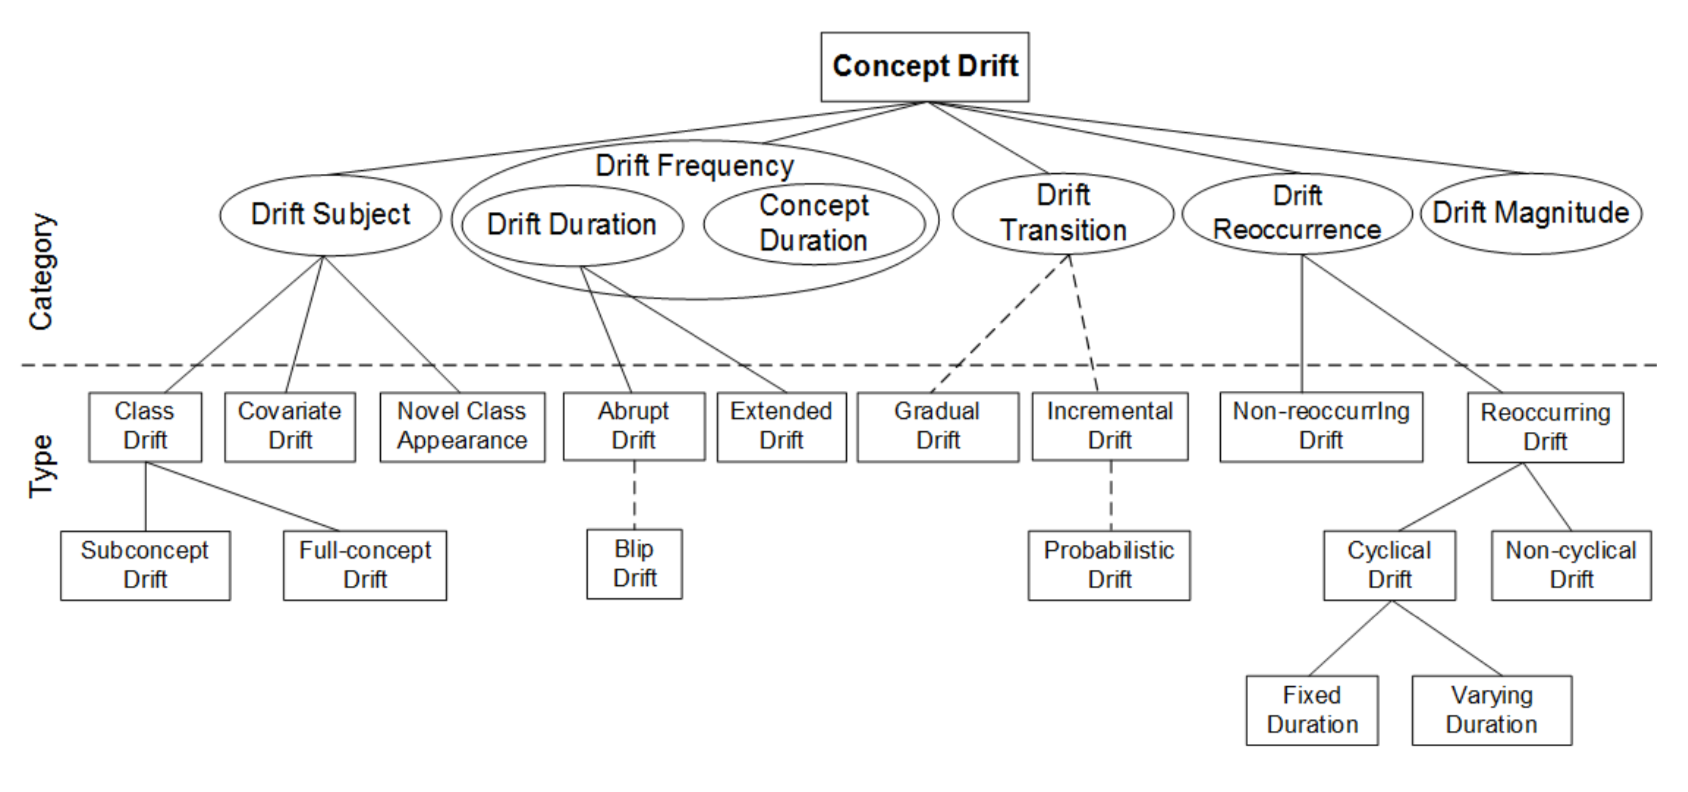
\includegraphics[width=\textwidth]{images/drift_taxonomy.png}
    \caption{Taxonomy of drift types. Solid lines denote mutually exclusive subcategories. Dashed lines denote non-mutually exclusive subcategories. Illustration originally appeared in Webb et al. \cite{characterizing_drift}.}
    \label{fig:drift_taxonomy}
\end{figure}


%-------------------------------------------------------------------
% RELATED WORK
%-------------------------------------------------------------------

\section{Related Work} \label{background:related_work}

There are broadly two approaches to handling concept drift. {\bf Blind} approaches do not explicitly model drift, instead allowing the model to gradually adapt to the new environment. {\bf Informed} approaches, instead employ {\bf drift detectors} to explicitly detect when concept drift has occurred so that the model can be retrained on data from the drift point onward \cite{gama_survey}.

A drift detector is an algorithm which predicts whether drift has occurred for a given data stream
\begin{equation}
    D(Z) \approx \begin{cases}
    1 & \text{if drift has occurred on $Z$} \\
    0 & \text{otherwise}
    \end{cases}
\end{equation}
The following are desirable properties for a drift detector:
\begin{itemize}
    % \item A detector should ideally be {\bf transparency} This enables practitioners to both understand the shortcomings of the model and identify when it is going wrong, and also should allow them to trust the system more, given they can actually see its internal mechanisms.
    \item {\bf Adaptiveness} The ability to detect when concept drift has occurred in a short span of time so that model retraining can commence quickly.
    \item {\bf Accuracy} The system should have a low rate of false-positives and false negatives, so that unnecessary training isn't invoked, and necessary training isn't neglected.
    \item {\bf Robustness} The system should be robust to noise.
\end{itemize}
We now present a survey of the field of concept drift detection research.

% \section{Theoretical Results Pertaining to Concept Drift}
% Holembold and Long (1991, 1994) provide an algorithm which is adaptable to drift up to a given extent.
% Kuh , Petsche, and Rivest (1991, 1994) provide an algorithm and theoretical guarantees for a maximum rate of drift. Their approach is based on the PAC framework.

\subsection{Early Algorithms}

Page \cite{CUSUM} introduced the field of change detection, the parent field of concept drift detection. Page proposed the Page-Hinkley Test (PHT), also known as CUSUM algorithm, in the context of industrial quality control. We imagine testing fixed-size samples of some product from various batches. The number of faulty products from batch $i$ is given by $x_i$. We would like to raise the alarm that the industrial process has gone awry whenever the following condition is met:
\begin{equation}
    \begin{cases}
        x_n > 1 & \text{or} \\
        x_n + x_{n-1} > 2 & \text{or} \\
        \vdots \\
        \sum_{i=0}^k x_{n-i} > k + 1 & \text{for some $k$}
    \end{cases}
\end{equation}
This is equivalent to recording the cumulative sum $S_n = \sum_{i=0}^n x_i$ and raising the alarm whenever
\begin{equation}
    S_n - \min_{i} S_i > h
\end{equation}
for some $h$. In practice, this means we need only keep two registers. First, $S_n$ which accumulates $x_i$, and $S_{min}$, which stores the minimum value of $S_i$ encountered so far.

% This equation can easily be adapted to detect significant deviations in both the positive and negative directions. CUSUM may therefore be used to detect change in any real-valued time series. It can also be used to detect changes in a binary-valued series, if the series is processed in batches, as in the motivating example. 

Work on concept drift often describes adaptations of CUSUM to the problem of concept drift detection \cite{barros_comparison}\cite{gama_survey}. These works cite the original paper by Page \cite{CUSUM}, making the author of these variations unclear. %I have elected to describe the original form of the algorithm as it is more elegant and theoretically justified than its variations.

The study of concept drift {\it per se} appears to originate with the STAGGER algorithm \cite{STAGGER}. This work was heavily influenced by cognitive psychology, so the original usage of ``concepts drift" denoted changes in conjunctive definitions of words. For example, a concept drift could be {\tt bachelor = unmarried AND man} changing to {\tt bachelor = unmarried AND woman}. This work also introduced the STAGGER dataset, which has become a standard benchmark in the field. 

The FLORA family of algorithms  \cite{FLORA}\cite{FLORA2}\cite{FLORA3} expanded the study of symbolic concept drift, and introduced many ideas to the field including recurring concepts, sliding windows of recent examples, and dynamic changes to the window size depending on the stability of the concepts. 

Klinkenberg and Joachim subsequently expanded the study of concept drift to real-valued domains \cite{SVM_detection}. Their approach was to train an SVM online, using a sliding window whose size is chosen to minimise generalisation error, which is estimated with the $\zeta\alpha$ metric. Although this approach was efficient and theoretically well motivated, it was tied specifically to SVMs, and so was not a general solution to the problem of concept drift detection.

The sequential probability ratio test (SPRT) \cite{SPRT} detects when a time series drifts from one distribution $P_1(z)$ to a new distribution $P_2(z)$. Let $z_1,z_2,\dots,z_n$ be some sequence. SPRT monitors the metric
\begin{equation}
  T_1^n = \log\frac{P_1(z_1,z_2,\dots,z_n)}{P_2(z_1,z_2,\dots,z_n)} = \sum_{i=1}^n \log\frac{P_1(z_i)}{P_2(z_i)}
\end{equation}
When $T_1^n>L$, for some parameter $L$, SPRT signals that drift has occurred.

\subsection{Drift Detection Method}

Drift detection method (DDM) \cite{DDM} maintains a running observed mean of the residual time series $p$. The uncertainty around the true error rate is estimated via a normal distribution (the true posterior is a beta distribution) with standard deviation $s=\sqrt{p(1-p)/i}$. A register of the lowest values of $p$ and $s$ are maintained, denoted $p_{min}$ and $s_{min}$. If $s+p>s_{min}+2\cdot s_{min}$, DDM emits a drift warning, and all new instances from that point are stored in a buffer. If $s+p>s_{min}+3\cdot s_{min}$, DDM emits a signal that drift has occurred, and the model is retrained on the instances in the buffer. 

RDDM \cite{RDDM} is a variant of DDM with periodic resets to become more reactive to changes in the error-rate. EDDM \cite{EDDM} is another variant, which monitors for changes in the distribution of {\it gaps} between errors, rather than changes in the error rate itself.

\subsection{Sliding Window Methods}

STEPD essentially approaches concept drift detection by testing the hypothesis ``the error-rate changed $n$ time steps ago for some fixed, and pre-set $n$" at each time step \cite{STEPD}. This is achieved by partitioning the data stream history into 1) a sliding window of the most recent $n$ values, and 2) the preceding values. The statistical test of equal proportions is then used to test whether the rates of the two partitions are significantly different.

FTDD , FPDD, and FSDD \cite{FTDD} are variants of STEPD, which uses Fischer's exact test %or the chi-square test 
in place of the test of equal proportions, because the latter is inappropriate for small or imbalanced data. 

WSTD is another variant, which uses the Wilcoxon rank sum statistical test instead of the test of equal proportions, and additionally limits the size of the second partition \cite{WSTD}.

PL (paired learners) is another sliding window method \cite{PL}. However, rather than testing for differences in error rates of a single model between the two partitions, it instead tests for differences in the error rates of two models. One model, the ``stable learner" is trained online on the entire data stream, and the other, the ``reactive learner" is trained only on the contents of the sliding window. If the proportion of instances in the window that are classified correctly by the reactive learner, but not the stable learner, exceeds some threshold, then drift is indicated.

FHDDM may be considered a hybrid of DDM and sliding window methods \cite{FHDDM}. At each time step the error rate in the sliding window is estimated. If this error rate significantly exceeds its lowest value, then drift is indicated.

SEQDRIFT2 \cite{seq_drift} uses the Bernstein bound to compare a window of the most recent instances with a reservoir of the preceding instances.

MDDM \cite{MDDM} uses both a sliding window {\it and} geometric or linear weighting, and uses the McDiarmid bound. It detects increases in the weighted error rate in the window.

\subsection{Adaptive Windowing}

A major flaw of the sliding window approaches is that they are brittle with respect to the window size parameter. If the window size is too large then there will be a large delay in the drift detection. If the window is too small then the detector will not be able to detect small drifts over random noise. ADWIN combats this problem by dynamically increasing or decreasing the window size \cite{ADWIN}. The authors explain:
\begin{displayquote}
    The idea is simple: whenever two ``large enough" subwindows of $W$ exhibit ``distinct enough" averages, one can conclude that the corresponding expected values are different, and the older portion of the window is dropped. In other words, $W$ is kept as long as possible while the null hypothesis ``$\mu_t$ has remained constant in $W$" is sustainable up to confidence $\delta$.
\end{displayquote}
This involves testing for drift at each time step in the window, which requires a multiple comparisons correction. One of the main advantages of ADWIN is that it provided theoretical guarantees on its false positive and negative rates.

SEED \cite{SEED} is another drift detection method which considers multiple drift points. Unlike ADWIN, the data are processed in batches or ``blocks", so most possible drift points are automatically excluded. When contiguous blocks are evaluated via the Hoeffding inequality to have the same rate, then the two are merged, thus eliminating one potential drift point.

\subsection{EWMA}

An exponentially weighted moving average (EWMA) \cite{EWMA} is an estimation of a variable $x$, which gives exponentially more weighting to more recent examples:
\begin{equation}
  \hat{x}_t = \lambda \hat{x}_{t-1} + (1-\lambda) x_t
\end{equation}
where $\lambda$ is the decay factor. EWMA is employed in several drift detection methods as it provides a way of estimating the current error rate of the model without knowing how far back in time a drift occurred. When the EWMA estimation of the error rate is significantly larger than the overall mean error rate, then we may conclude drift has occurred. ECDDM is a straightforward application of EWMA to concept drift detection, deriving p-values from a lookup table \cite{ECDDM}. LFR also uses EWMA, although p-values are derived from Monte Carlo estimation \cite{LFR}.

\subsection{HDDM}

Fr{\'\i}as-Blanco et al. \cite{HDDM} cast the drift detection problem as follows. There are $n$ examples $x_1,\dots,x_n$, and a hypothesised drift point $d$. The instances before the drift point are denoted $X=x_1,\dots,x_{d-1}$, and their mean is denoted $\mu_X$. Similarly, those instances after the drift point are denoted $Y=x_d,x_{d+1},\dots,x_n$, and their mean $\mu_Y$. These means are estimated using either the sample average or exponentially weighted average. Depending on which estimator is used, the method is known as HDDM$_A$ or HDDM$_W$. The estimations are denoted $\hat{\mu}_X$ and $\hat{\mu}_Y$, respectively. The authors derive bounds for $P(\hat{\mu}_X+\epsilon < \hat{\mu}_Y|\mu_X \ge \mu_Y)$ and $P(\hat{\mu}_X > \hat{\mu}_Y|\mu_X+\epsilon < \mu_Y)$, thus bounding the false positive and false negative rates, respectively.

This is incorporated into an online drift detection algorithm as follows. At time $t$, the hypothesised drift point is set to $d=t$, and is fixed at this value until enough instances are accumulated to the right of the drift point that either $P(\hat{\mu}_X+\epsilon < \hat{\mu}_Y|\mu_X \ge \mu_Y)$ is statistically insignificant, in which case a drift is signalled, or $P(\mu_X+\epsilon < \mu_Y)$ is statistically insignificant, in which case $d$ is set to the current time step. A major advantage of HDDM is that the derived bounds do not assume that the data stream to be monitored is Bernoulli, so can be used to detect drift on real-valued loss streams.

\subsection{Region Drift}

Most of the drift detectors discussed so far have supposed that when concept drift occurs, all the data before the drift becomes irrelevant. Liu et al. \cite{LLD} introduced the notion of {\bf region drift}, in which concept drift only affects a ``region" of instance space. Thus all the data outside of this region from before the drift can be reused when retraining the model. The authors present a new drift detector, local drift degree (LLD), which processes data in batches and uses the nearest neighbour methods to determine if drift has occurred in each region since the previous batch.

\subsection{Data Batches}

Degree of drift (DoF) \cite{DoF} considers data in batches. If the most recent two batches have a heterogeneous Euclidean/overlap metric (HEOM) which is $s$ standard deviations above the mean of past batches, then drift is indicated.

\subsection{Unbalanced Classes}

Wang et al. \cite{DDM-OCIa}\cite{DDM-OCIb} argue that most drift detectors, which detect concept drift via monitoring for increases in the error rate are unsuitable for data streams with unbalanced classes, because
\begin{quote}
  the  minority class  contributes  too  little  to  these  performance  measures compared  to  the  majority  class [and]  too  few  examples from the minority classes can make the time arbitrarily long until  the  concept  drift  is  detected.
\end{quote}
Wang et al. thus propose drift detection method for online class imbalance (DDM-OCI). This monitors for decreases in the recall of the minority class, rather than decreases in the overall accuracy of the model.

Linear four rates (LFR) \cite{LFR} expands on this idea. In addition to monitoring the recall of the minority class, it also monitors the recall of the majority class and the precision of both. It uses an EWMA-style \cite{EWMA} estimator with lookup tables to detect changes in these rates.

PerfSim \cite{perfsim} similarly monitors all the components of the confusion matrix, and uses the cosine similarity test to detect changes between batches of data. CSDD \cite{CSDD} uses the same test, but uses a sliding window rather than batches of data.

\subsection{Bayesian Concept Drift Detection}

Many researchers have proposed Bayesian approaches to change point detection, a problem closely related to concept drift detection. Barry and Hartigan \cite{barry_hartigan} derived an $O(n^3)$ algorithm for detecting {\it multiple} change points within a time series. Fearnhead \cite{fearnhead} developed an $O(n^2)$ algorithm to achieve the same task. 

Adams and MacKay \cite{adams_mackay} adopted a Bayesian approach to change point detection for online contexts. This approach considers a hypothesis space of $l=1, l=2, \dots$, where $l=i$ indicates that a drift point occurred $i$ time steps in the past. At each new time step, the posterior $\Pr(l=i)$ for each $i$ is recalculated.

Bach and Maloof \cite{BCMC} adopted the Adams-MacKay approach to concept drift adaptation. They proposed the Bayesian conditional model comparison (BCMC) algorithm, which makes predictions according to an ensemble of Bayesian learners, one for each value of $l=i$. The models are weighted according to the $\Pr(l=i)$ posteriors. The authors also propose a more efficient algorithm which approximates BCMC, called the pruned Bayesian conditional model comparison (PBCMC).

% \subsection{Ensemble approaches}
% ELM \cite{ELM}


% \subsection{Expeirments}

% \cite{barros_comparison}


%-------------------------------------------------------------------
% CONCLUSION
%-------------------------------------------------------------------

\section{Conclusion} \label{background:conclusion}

With some abstraction, we can consider drift detection methods of consisting of three components. First is the method of generating drift point candidates. The common approaches are using a {\it sliding window}, in which case the candidate drift point is the start of the window, {\it aggregation}, in which case the data stream is aggregated into blocks and the spaces between these blocks are used as drift point candidates, {\it batching}, in which the spaces between batches of data are drift point candidates, and {\it thresholding}, in which case the candidate drift point is derived by monitoring for a summary statistic exceeding some threshold.

The second component of a drift detector is a statistical test. Many detectors make use of Hoeffding's test, Bernstein's test, McDiarmid's test, Fischer's exact test, or the cosine test. 

The third component is the operationalisation of concept drift. The general problem of concept drift detection is virtually insoluble in its most general form, so drift detectors operationalise the problem to make it tractable. The most common operationalisation is to detect increases in the error rate of the model. Other approaches include monitoring for increases in the precision and recall.
All the existing drift detectors we have surveyed are summarised according to these components in Table \ref{tab:drift_detectors}.

\begin{table}[]
    \centering
    \caption{Summary of existing drift detectors}
    \label{tab:drift_detectors}
    \begin{tabular}{|l|l|l|l|}
         \toprule
         Detector & Drift Points & Statistical Test & Operationalisation  \\
         \midrule
         ADWIN & aggregation & Hoeffding & Accuracy \\
         CSDD & cosine & batches & Recall, Precision \\
         CUSUM & threshold & - & Accuracy \\
         DDM & threshold & - & Accuracy \\
         DDM-OCI & threshold & - & Recall \\
         DoF & batches & - & Accuracy \\
         ECDDM & threshold & - & Accuracy \\
         EDDM & threshold & Hoeffding & Accuracy \\
         FHDDM & window & Hoeffding & Accuracy \\
         FLORA & - & - & Accuracy \\
         HDDM & window & Hoeffding & Accuracy \\ 
         LDD & batches & - & Accuracy \\
         LFR & threshold & - & Recall, Precision  \\
         MDDM & window & McDiarmid & Accuracy \\
         PerfSim & window & cosine & Recall, Precision \\
         PL & window & - & Accuracy \\
         RDDM & threshold & Hoeffding & Accuracy \\
         SEED & Blocks & Hoeffding & Accuracy \\ 
         SeqDrift2 & window & Bernstein & Accuracy \\
         SPRT & threshold & - & - \\
         STAGGER & - & - & Accuracy \\
         STEPD & window & - & Accuracy \\
         \bottomrule
    \end{tabular}
\end{table}








